\section{Durchführung}
\label{sec:Durchführung}
In diesem Versuch werden, wie in \autoref{sec:Ziel} bereits beschrieben, die Magnetfelder verschiedener Spulenkonstellationen gemessen. Die Messmethoden dazu werden im folgenden 
Kapitel erläutert. Zuerst werden jedoch die Vorbereitungsaufgaben diskutiert.
\subsection{Vorbereitungsaufgaben}
\label{subsec:VBA}
In der ersten Vorbereitungsaufgabe sollte die magnetische Flussdichte im Zentrum eines Helmholtzspulenpaares berechnet werden. Dies geschieht nach \autoref{eqn:Helmholtz}.
Die Spulen des Helmholtzspulenpaares haben einen Durchmesser $d = 125\unit{\milli\metre}$, der Abstand der Spulen beträgt $x = \sfrac{d}{2}$ gilt. Das Spulenpaar 
wird von einem Strom mit $1 \: \unit{\ampere}$ durchflossen. Mit diesen Werten und der magnetischen Feldkonstante 
$\mu_0 = 1.2566\cdot 10^{-6} \unit{\newton\per\ampere\squared}$\cite{scipy} ergibt sich $B(0) = 0.71\unit{\milli\tesla}$ für das Magnetfeld. 

Im zweiten Teil der Vorbereitung sollten die Begriffe Dia- Para- und Ferromagnetismus erklärt werden. 
\subsubsection{Diamagnetismus}
\label{subsubsec:DIA}
Diamagnetische Stoffe sind durch eine Permeabilität $\mu_{\text{r}} < 1$ ausgezeichnet. Liegt ein äußeres Magnetfeld an, bilden sie ein Gegenfeld, welches das anliegende Magnetfeld
abschwächt. Ohne äußeres Magnetfeld sind diamagnetische Stoffe nicht magnetisch. 
\subsubsection{Paramagnetismus}
\label{subsubsec:PARA}
Paramagnetische Stoffe verhalten sich gegenteilig. Sie sind ebenfalls ohne äußeres Magnetfeld nicht magnetisch, aber erzeugen in einem äußeren Magnetfeld ein paralleles Feld.
Die Felder überlagern sich, was zur Folge hat, dass das Gesamtfeld im Inneren des paramagnetischen Materials verstärkt wird. Paramagnetische Stoffen zeichnen sich durch eine 
Permeabilität $\mu_{\text{r}} > 1$ aus. 
\subsubsection{Ferromagnetismus}
\label{subsubsec:FERRO}
Ferromagnetische Stoffe können ohne ein äußeres Magnetfeld eigene permanente Mangetfelder besitzen. Diese bilden sich, da die einzelnen Atome jeweils magnetische Momente besitzen, welche 
dazu neigen sich parallel zueinander auszurichten. Die ferromagnetischen Stoffe, die kein Magnetfeld besitzen, werden meist sehr stark von einem äußeren Pol angezogen. Solche Stoffe 
sind durch eine Permeabilität $\mu_{\text{r}} >> 1$ gekennzeichnet. Eine weitere wichtige Eigenschaft solcher Stoffe ist, dass sie sich magnetisieren lassen. Diese Magnetisierung findet
durch ein äußeres Magnetfeld statt und bewirkt, dass ein ferromagnetischer Stoff sein eigenes Magnetfeld aufbaut oder verändert. Hysteresekurven, wie zum Beispiel die in \autoref{fig:PlotHysterese},
geben die Magnetisierung gegen eine gewissen Größe an. In diesem Fall wird sie gegen den Strom angegeben.
\subsection{Messung des Magnetfeldes einer langen Spule}
\label{subsec:D_Lange_Spule}
Zur Messung des Magnetfeldes einer langen Spule benötigt man die Spule selbst, eine logitudinale Hall-Sonde und einen Stromgenerator. Zunächst wird die Spule an den Generator angeschlossen.
Der Generator wird dann so eingestellt, dass die Spule von circa $1 \unit{\ampere}$ durchflossen wird. Dann befestigt man die Hall-Sonde in einem Gestell, sodass immer möglichst auf der
gleichen Achse gemessen wird. Man wählt einem Messnullpunkt und schiebt die Hallsonde dann langsam in die Spule ein. Dabei wird die relative Auslenkung zum Messnullpunkt und die Magnetfeldstärke 
an diesen Stellen gemessen. Aus Symetriegründen reicht es aus bis zur Mitte der Spule zu messen.
\begin{figure}
    \centering
    \caption{In diesem Bild ist die verwendete lange Spule abgebildet. Die Länge der Spule wurde graphisch auf $16.4 \: \unit{\centi\metre}$ bestimmt.}
    \label{fig:Aufbau_lange_Spule}
    \includegraphics[width=0.7\textwidth]{content/LangeSpule.jpg}
\end{figure}
\subsection{Messung des Magnetfelds eines Spulenpaares}
\label{subsec:D_Spulenpaar}
Für diese Messung benötigt man ein Helmholtzspulepaar, dessen Abstand man variieren kann. Außerdem benötigt man eine transversale Hall-Sonde zur Messung des Magnetfeldes. Zunächst
werden die beiden Spulen in Reihe an einen Generator angschlossen, sodass beide Spulen gleichsinnig vom Strom durchflossen werden. Nun muss zunächst ein Abstand zwischen den Spulen 
festgelegt werden. Die Hall-Sonde wird, wie in \autoref{fig:Aufbau_Spulenpaar} dargestellt ist, oben in die Führung eingesetzt. Dadurch ist garantiert, dass man entlang einer Achse misst.
Dann werden in sinnvollen Abständen Messungen durchgeführt. Dabei wird sowohl der Bereich zwischen den Spulen als auch der Bereich außerhalb der Spulen gemessen. Dies wird für 3 unterschiedliche 
Längen wiederholt.
\begin{figure}
    \centering
    \caption{In diesem Bild ist der Versuchsaufbau zum Helmholtzspulenpaar dargestellt.\cite{v308}}
    \label{fig:Aufbau_Spulenpaar}
    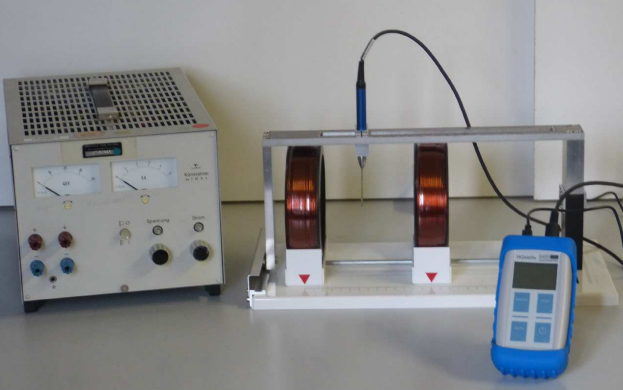
\includegraphics[width=0.7\textwidth]{content/HelmHoltzAufbau.PNG}
\end{figure}
\subsection{Messung des Magnetfeldes einer Toroid-Spule zur Bestimmung der Hysteresekurve}
\label{subsec:D_Hysterese}
Für diese Messung wird eine Toroidspule und eine transversale Hall-Sonde benötigt. Die Hall-Sonde wird über eine Vorrichtung in den Luftspalt der Toroidspule gehalten. Die Toroidspule
wir an einen Generator angeschlossen. Bevor dieser eingeschaltet wird, muss die Spule möglichst gut entmagnetisiert werden. Dann wird der Generator eingeschaltet. Nun wird der Strom
der Spule langsam hochgeregelt, wobei immer die dazugehörigen Feldstärken notiert werden. In dieser Messung können $1\unit{\ampere}$-Schritte gemacht werden. Es wird gemessen bis die 
gesamte Hysteresekurve abgemessen wurde. Das bedeuetet nach Beginn der Messung wird der Generator zunächst bis zu $10\unit{\ampere}$ hochfahren und auch wieder bis zur $0$ runtergeregelt.
Um dann in den negativen Bereich zu gelangen wird die Verkabelung umgedreht. Dann wird der gleiche Messprozess nochmal durchgeführt. Danach wird nochmals umgepolt und lediglich ein mal 
bis $10\unit{\ampere}$ hochgemessen. Nun wurde die gesamte Hysteresekurve abgemessen.
\begin{figure}
    \centering
    \caption{Dies ist ein Bild des Versuchaufbaus zur Toroidspule.\cite{v308}}
    \label{fig:Aufbau_Toroid}
    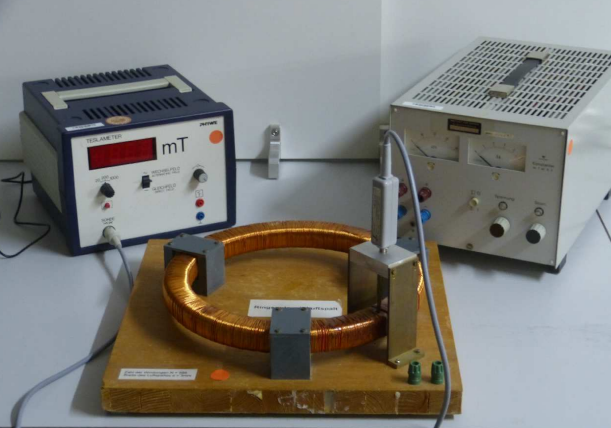
\includegraphics[width=0.7\textwidth]{content/RingSpuleAufbau.PNG}
\end{figure}